\section{Security and Risk Management} \label{section: SARM}
This chapter provides an introduction to security and risk management by covering key concepts such as data compliance, identity and access management (IAM), data encryption, and data backups. 

This chapter is not intended to be a comprehensive handbook for implementing proper security measures, but rather as an overview of the security measures to consider when developing a strategy for storing and accessing sensitive information.

\subsection{Data Compliance}

\begin{itemize}
    \item HIPAA Compliance \cite{USDHHS}
    \item UHM Compliance
    \item RCUH Compliance
    \item TASI Compliance
    \item State of Hawaii Compliance
\end{itemize}

\subsection{Identity and Access Management (IAM)}
Identity and Access Management (IAM) is a security practice that safeguards sensitive information by allowing only authorized individuals to access confidential resources and data \cite{AWS}. 

Identity management looks to confirm that an accessing user is who they say they are, whilst access management uses a users identity to determine which resource they are allowed to access. 

IAM components can be classified into four major categories: authentication, authorisation, user management, and central user repository.

\subsubsection{Authentication}\label{2.2.1}
Authentication is a component of IAM in which a user is required to provide sufficient credentials to gain access to an application system. 

Sufficient credentials for accessing sensitive healthcare information are defined as authentication methods that comply with the HIPAA Security Rule (Section 5.1). The HIPAA Security Rule requires covered entities to implement multi-factor authentication or an equivalent authentication method for accessing ePHI.

According to HIPAA, the multi-factor authentication method must use two of the following three elements:

\begin{itemize}
    \item Something you know (Password or PIN)
    \item Something you have (Smart Card or Security Token) 
    \item Something you are  (Fingerprint or Facial Recognition)
\end{itemize}

Two new additional standards are not required but provide additional authentication methods:

\begin{itemize}
    \item Somewhere you are (IP Address or Geo-location)
    \item Something you do (Signature or Gesture)
\end{itemize}

Once a user is authenticated, a session is created to allow the user to interact with the application system. The session will remain open until the user's task is completed or through termination by other means (e.g., timeout). By centrally maintaining the session of a user, the authentication module can provide single sign-on services. 

Single sign-on (SSO) is a mechanism that allows users to authenticate once and access multiple systems or applications without having to re-enter their credentials. SSO simplifies access control and user permissions by providing a centrally managed solution for user authentication policies across all systems. There are several options when deciding on a SSO solution. (e.g., LDAP, OAuth, SAML, RADIUS, PKI, etc).

\subsubsection{Authorization}
Authorization is a component of IAM in which a user is given permission to access a particular resource. 

This component comes after a user has successfully authenticated to an application system with sufficient credentials. Authorization is performed by checking the resource access request (e.g., web-based application URL), against an IAM policy store and is the core module that implements Role-Based/Attribute-based, access control. 

\begin{itemize}
    \item Role-Based Access Control (RBAC) is a method of access control that assigns roles to users  and access permissions to those roles in order to provide a centrally managed solution for authorization. 
    \item Attribute-Based Access Control (ABAC) is a method of access control that assigns permissions based on a user's attributes (e.g., job title, location, department). 
\end{itemize}

The authorization model can provide more complex access control policies other than user role/groups and user attributes (e.g., access channels, time, resource requested, external data, business rules). 

\subsubsection{Central User Repository}
The Central User Repository (CUR) stores and delivers identity information in order to verify credentials submitted from clients. Identity information is equivalent to user account information (e.g., usernames, passwords, etc). The most common CUR protocol is the Lightweight Directory Access Protocol (LDAP). 

LDAP is a protocol for accessing and maintaining distributed directory information services over an Internet Protocol network in order to provide a centrally managed authentication and authorization solution for application systems. 

LDAP allows system administrators to manage user accounts, configure access and permissions, and monitor and audit user activity.

\begin{figure}[H]
    \centering
    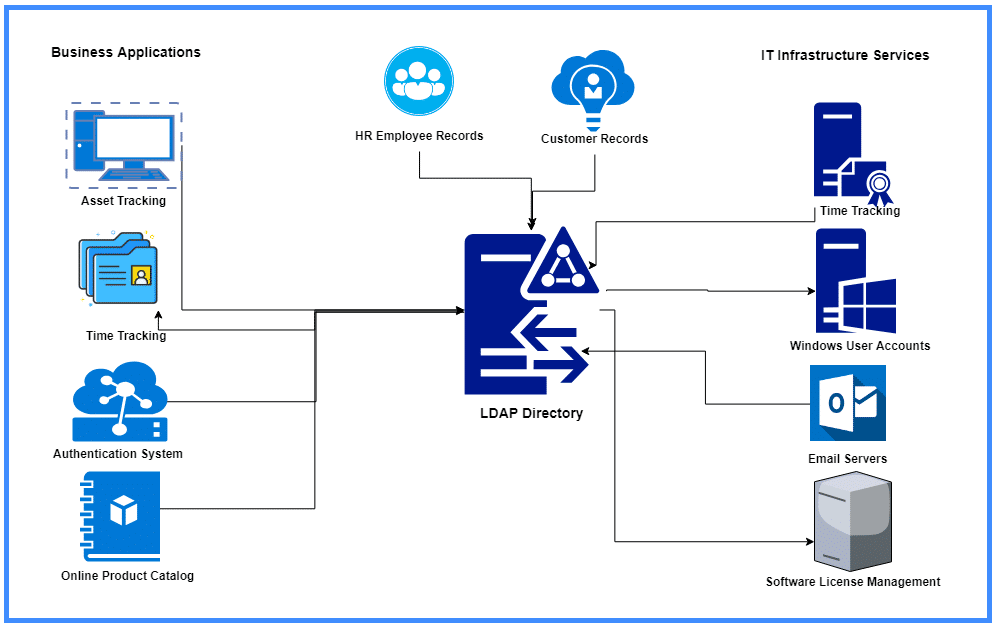
\includegraphics[scale = 0.6]{images/LDAP.png}
    \caption{\href{https://doubleoctopus.com/security-wiki/protocol/lightweight-directory-access-protocol/}{\textcolor{black}{Lightweight Directory Access Protocol}} \cite{SecretDoubleOctopus}}
    \label{LDAP}
\end{figure}

When designing an LDAP directory, it is important to consider the principle of least privilege. The principle of least privilege is a design principle where each user or service is only given the necessary permissions to perform their intended tasks, and no more. Unauthorized users should not access important data or systems. The principle of least privilege should also be considered when designing security groups and access control lists, as unauthorized users must not have access to sensitive information.

\subsubsection{User Management}

User Management is the component of IAM that covers the creation and maintenance of user accounts, account identity, and account privileges \cite{Billmath}. 

Identity creation and maintenance is controlled by the set of administrative functions such as user life-cycle management, role/group management, and user/group provisioning. User life-cycle management controls the lifespan of user accounts from account provision to account deprovision. Role/group management and user/group management is used for user authorization (Section \ref{2.2.1}). 

Onboarding, maintenance, and off-boarding are the three components of user life-cycle management. 

\begin{enumerate}
    \item On-boarding Process:
        \begin{itemize}
            \item Account authentication for relevant systems and applications.
            \item Verification of tenant identity.
            \item Setting up multi-factor authentication.
            \item Domain and network access configuration.
            \item Training for new tenants on how to use the systems and applications they have access to.
        \end{itemize}
    \item Maintenance Process:
        \begin{itemize}
            \item Regular review of tenant access privileges to ensure that they align with the tenant's job function and level of responsibility.
            \item Management of access requests and approvals to ensure that access is only granted to authorized tenants.
            \item Management of tenant accounts and passwords, including password expiration policies and periodic password resets.
            \item Monitoring and auditing tenant activity to detect for potential security threats.
            \item Provisioning of additional access or permissions based on changes to the tenant's role or job function.
        \end{itemize}
    \item Off-boarding Process:
        \begin{itemize}
            \item Revocation of tenant access to all systems and applications once life-cycle is expired. 
            \item Archiving or removal of tenant data in accordance with the organizations (e.g., TASI, RCUH, UHM, etc.) policies and regulatory requirements.
            \item Review of tenant access to ensure that no data or resources have been left behind.
            \item Disabling or revocation of any credentials associated with the tenant's access.
            \item Notification of relevant stakeholders about the tenant's departure.
        \end{itemize}
\end{enumerate}

\subsection{Data Encryption}

Data Encryption is a security practice that safeguards sensitive information by transforming the data into an unreadable format that can only be deciphered with the appropriate decryption key \cite{IBM}. 

HIPAA Security Rule (Section 5.1) requires covered entities to implement a mechanism to encrypt and decrypt ePHI based on the assessment of risks to the confidentiality, integrity, and availability of the ePHI. 

\begin{itemize}
    \item Data At-Rest is data that is stored in storage devices (e.g., disk, tape, USB drives, non-votalite storage, etc) and is not being used or transmitted.
    \item Data In-Transit is data that is transmitted over a network (e.g., file transfers, emails, instant messages). HIPAA requires the use of secure transmission protocols (e.g., SSL, TLS) for transmitting ePHI over public networks. 
\end{itemize}

\subsection{Data Backup}

A Data Backup is a copy of data that is used for data restoration in the case of data loss, data corruption, or other data-related disasters.

\begin{itemize}
    \item Recovery Point Objective (RPO) is the maximum amount of data – as measured by time – that can be lost before data loss exceeds what is acceptable to an organization.
    \item Recovery Time Objective (RTO) is the maximum tolerable length of time that a system (e.g., can be down after a failure or disaster occurs. 
\end{itemize}

\subsection{Vulnerability Assessment}
A Vulnerability Assessment is the process of identifying vulnerabilities in a system to assess potential security risks \cite{Goel}. 

It involves scanning the system for known weaknesses, misconfigurations, or software vulnerabilities that could be exploited by bad actors. By conducting regular vulnerability assessments, organizations can proactively identify areas of weakness and take appropriate measures to mitigate potential threats.

The assessment typically follows these steps: 

\begin{enumerate}
    \item Vulnerability Scan:
    \begin{itemize}
        \item Utilizing automated tools to scan an organization’s IT environment to identify vulnerabilities and weaknesses.
    \end{itemize}
    \item Vulnerability Analysis:
    \begin{itemize}
        \item Determine the severity and impact on the system's security. Prioritize the vulnerabilities based on the level of risk.
    \end{itemize}
    \item Risk Assessment:
    \begin{itemize}
        \item Prioritize the remediation efforts based on the level of risk associated with each vulnerability.
    \end{itemize}
    \item Remediation Planning:
    \begin{itemize}
        \item Develop a plan to address the identified vulnerabilities. 
    \end{itemize}
    \item Ongoing Monitoring:
    \begin{itemize}
        \item Vulnerability assessments should be conducted on a regular basis to ensure that the system remains secure over time.
    \end{itemize}
\end{enumerate}

\subsection{Penetration Testing}
Penetration Testing, also known as ethical hacking, is a simulation of real-world attacks on a system to evaluate the security of a system \cite{Goel}.
\begin{enumerate}
    \item Planning:
    \begin{itemize}
        \item Defining the penetration test objectives and identifying the target system.
    \end{itemize}
    \item Reconnaissance:
    \begin{itemize}
        \item Gathering available information about a system through passive methods.
    \end{itemize}
    \item Vulnerability Assessment:
    \begin{itemize}
        \item Identify and assess the vulnerabilities in a target system using automated tools.
    \end{itemize}
    \item Exploitation:
    \begin{itemize}
        \item Exploit the identified vulnerabilities to gain unauthorized access, escalate privileges, or compromise sensitive data.
    \end{itemize}
    \item Post-Exploitation and Reporting:
    \begin{itemize}
        \item A detailed report is generated to show the vulnerabilities discovered, how it was exploited, and how to remediate them.
    \end{itemize}
\end{enumerate}
